%!TEX TS-program = xelatex
%!TEX root = ../../maxwell2018thesis.tex

\chapter[Modelling SERP Level Stopping Behaviours]{Modelling~\gls{acr:serp} Level\\Stopping Behaviours}\label{chap:serp}
In Chapters~\ref{chap:snippets} and~\ref{chap:diversity}, we conducted two user studies that examined effects of searcher behaviour and performance under different contexts. Interaction data from these studies were then used to ground simulations of interaction that examined how each of the twelve different stopping strategies performed and approximated real-world searcher stopping behaviours. We now turn our attention towards providing a complete answer to our first high-level research question, \darkblueboxbold{HL-RQ1}.

\begin{itemize}
    \item[]{\darkblueboxbold{HL-RQ1} How can we improve searcher models to incorporate different stopping decision points?}
\end{itemize}

In order to address this research question, we presented in Chapter~\ref{chap:csm} the~\glsfirst{acr:csm}, a conceptual, high level model of the search process. The~\gls{acr:csm} introduced the~\gls{acr:serp} level stopping decision point, motivated by informations scent (refer to Section~\ref{sec:stopping_background:theoretical:ift}). This new stopping decision point allows a simulated searcher to \emph{abandon} a~\gls{acr:serp} if a general \emph{overview} of the given~\gls{acr:serp} if the results, from a glance, did not appear to provide promising results. With the definition of the~\gls{acr:csm} partially satisfying \darkblueboxbold{HL-RQ1}, we in this chapter provide results of an empirical, simulated study of the new stopping decision point. This study provides evidence that the inclusion of this new stopping decision point does indeed improve simulated searcher performance, and offers closer approximations to how real-world searchers actually behaved.

\section{Motivation and Research Questions}\label{sec:serp:background}
With the background work for this chapter largely outline in Sections~\ref{sec:stopping_background:theoretical:ift} and~\ref{sec:csm:stopping}, this section provides a refresher of the motivation behind the inclusion of the third, new~\gls{acr:serp} level stopping decision point. We begin with the concept of~\gls{acr:serp} abandonment, before considering how~\glsfirst{acr:ift} provides strong theoretical motivation.

The concept of the new~\gls{acr:serp} level stopping decision point revolves around the concept of~\gls{acr:serp} abandonment, when a searcher fails to click on any of the results returned for a given query~\citep{diriye2012abandonment, hassan2013serp_abandonment}. This may be for a variety of different reasons (both good and bad) -- the primary motivator for this study considers the notion of bad abandonment, where searchers abandon a~\gls{acr:serp} because they are dissatisfied by the results returned~\citep{hassan2013serp_abandonment}.

\begin{figure}[t!]
    \centering
    \resizebox{1\hsize}{!}{
    \includegraphics{figures/ch9-csm.pdf}}
    \caption[The~\glsfirst{acr:csm} and~\gls{acr:serp} stopping point]{The~\glsfirst{acr:csm}, highlighting the stopping decision point (by an asterisk\emph{*}, with the~\gls{acr:serp} examination component also highlighted within the blue rectangle) that is examined in detail in this chapter. Refer to Section~\ref{sec:csm:flow} for an in-depth explanation of the model.}
    \label{fig:csm_ch9}
\end{figure}

Motivated by \emph{information scent} and the \emph{patch model} -- both part of~\glsfirst{acr:ift}\footnote{Refer to Section~\ref{sec:stopping_background:theoretical:ift} on page~\pageref{sec:stopping_background:theoretical:ift} for a detailed explanation of the patch model.} --~\cite{pirolli1999ift} argue that information seekers are like animals foraging in the wild, and as such will follow a scent to find food. As discussed previously, information seekers have been shown to follow a series of \emph{proximal cues} provided by~\gls{acr:serp} components such as hypertext links, titles, snippets and thumbnails to help locate relevant information~\citep{pirolli1995ift, pirolli1999ift, chi2001information_scent, oltston2003scenttrails, pirolli2007ift}. For example,~\cite{card2001scent_graphs} found that when navigating through webpages, searchers were more likely to leave when the information scent provided on a page began to decline. Work by~\cite{wu2014information_scent} discussed a user study where low, medium and high scent~\glsplural{acr:serp} were created by changing the number and distribution of relevant items on the page -- thus altering the proximal cues provided. Those interacting with high scent~\glsplural{acr:serp} examined more content and went to greater depths compared to those who utilised low scent~\glsplural{acr:serp}. Further work by~\cite{ong2017scent_behaviour} -- and indeed the user study reported in Section~\ref{chap:snippets:user} -- all confirm that modifying the scent of a~\gls{acr:serp} does indeed alter a searcher's stopping behaviour.

For this chapter, we operationalise the information scent as the performance of a given~\gls{acr:serp}, examining how the new~\gls{acr:serp} level stopping decision point within the searcher model -- as shown in Figure~\ref{fig:csm_ch9}\footnote{Further information on the~\glsfirst{acr:csm} can be found in Chapter~\ref{chap:csm}, starting on page~\pageref{chap:csm}.} -- affects searcher, stopping and overall performance. This is achieved by enumerating a series of different~\gls{acr:serp} level stopping strategies, allowing us to operationalise the new stopping decision point in several ways. As such, we pose two key research questions to be addressed in this chapter.

\begin{itemize}
    \item[]{\darkblueboxbold{RQ1} Does incorporating a~\gls{acr:serp} level stopping decision point lead to higher overall performance?}
    \item[]{\darkblueboxbold{RQ2} Does incorporating a~\gls{acr:serp} level stopping decision point lead to better approximations of searcher stopping behaviour?}
\end{itemize}

Taken together, the answers to these research questions will in turn provide a complete answer to allow us to address high level \darkblueboxbold{HL-RQ1}, allowing us to determine whether the inclusion of this additional~\gls{acr:serp} level stopping decision point does improve on the current state-of-the-art. In the next section, we outline the methodology undertaken to address the aforementioned research questions.

\section{Methodology}
In order to address the two research questions posed above, we followed our simulation methodology, outlined in our general methodology chapter. This is detailed in Section~\ref{sec:method:simulation} on page~\pageref{sec:method:simulation}. A variety of different simulation components that mapped to individual components of the~\gls{acr:csm} were left unchanged from the general methodology; this section details the changes to our experimental setup, the key component being the~\gls{acr:serp} level stopping decision point was operationalised for this study.

In this section, we therefore outline:

\begin{itemize}
    \item{the different~\gls{acr:serp} level stopping decision point strategies that were trialled, including the introduction of a new probability of examining a~\gls{acr:serp} (Section~\ref{sec:serp:method:serp_dp});}
    \item{a discussion of the different interaction probabilities and costs that were used for this study (Section~\ref{sec:serp:method:probscosts});}
    \item{an enumeration of the different result summary level stopping strategies trialled for this study (Section~\ref{sec:serp:method:snippet}); and}
    \item{a summary of the other components of the~\gls{acr:csm} that were instantiated in a different way as outlined in the general methodology (Section~\ref{sec:serp:method:other}).}
\end{itemize}

\subsection{SERP Decision Making}\label{sec:serp:method:serp_dp}
This section discusses the various ways in which we implemented this new stopping decision point, allowing us to determine whether it leads to any improvements in overall search performance and better approximations to real-world searcher stopping behaviours. As a searcher can only obtain an impression of the overall quality of a~\gls{acr:serp} from what he or she can see \emph{at a glance,} we begin this section with a discussion on the \emph{size of the browser's viewport.}

\blueboxbold{Considering Browser Viewport Size}
As we discussed previously in Section~\ref{sec:serp:background}, real-world searchers are able to infer the quality (and perhaps relevance) of a given page or~\gls{acr:serp} through the examination of various proximal cues~\citep{chi2001information_scent}. Such cues are not considered in this work; instead, we rely upon more simplistic means to implement the stopping decision point. One aspect of presentation we do consider in this chapter is the \emph{size of the browser's viewport}. A~\gls{acr:serp} is typically larger than the viewport it is displayed within, which leads to the inclusion of scrollbars. Results can only be seen \emph{above-the-fold}, or what is visible within the viewport. We argue that a searcher can infer the quality of the~\gls{acr:serp} from the initial view they are presented with, and thus incorporate a \emph{viewport size} ($v_{size}$) variable in our simulations of interaction. A searcher can only judge what they can see. This variable can vary between the different interfaces we trialled -- for example, longer snippet text results in fewer result summaries being displayed in the initial view. By using a fixed-size popup window in the two user studies (as discussed in Section~\ref{sec:methodology:user:interface}), we were able to manually check the number of result summaries displayed within the popup window, and use these values to provide more extensive grounding to the new stopping decision point.

\begin{wrapfigure}[13]{r}{0.45\textwidth}
    \begin{center}
    \vspace*{-9mm}
    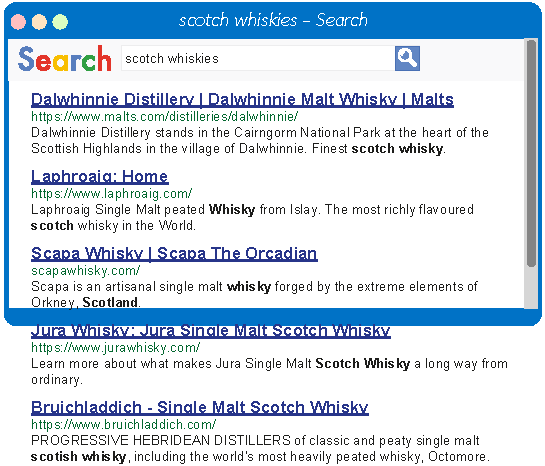
\includegraphics[width=1\textwidth]{figures/ch6-viewport.pdf}
    \end{center}
    \vspace*{-2mm}
    \caption[Viewport cutoff example]{The~\gls{acr:serp} viewport threshold. In this example, three result summaries are visible, with two present but outwith the viewport. Therefore, \emph{v\textsubscript{size}=3}. Cheers!}
    \label{fig:viewport_cutoff}
\end{wrapfigure}

For simulations of interaction reported in this chapter, we use different values of $v_{size}$ over the experimental interfaces reported in Chapter~\ref{chap:snippets} only. As we varied the length of result summaries across the four experimental interfaces (from \blueboxbold{T0} to \blueboxbold{T4}), this would impact upon the number of result summaries visible in the initial view (used for obtaining an impression of the overall~\gls{acr:serp}). Longer result summaries would mean that fewer would be presented within a viewport of the same size, compared to shorter result summaries. However, result summary lengths were not modified under the experimental conditions trialled in Chapter~\ref{chap:diversity}. This means that $v_{size}$ would remain constant.

\blueboxbold{Definition: Low vs. High Scent} Given a~\gls{acr:serp}, would it constitute as \emph{low scent} or \emph{high scent?} For this chapter, we follow the work of~\cite{wu2014information_scent}. In their study, the authors state that a low scent~\gls{acr:serp} offers little or no relevant content. Definitions by~\cite{wu2014information_scent} and~\cite{hassan2013serp_abandonment} define a poor scented~\gls{acr:serp} as $P@10=0.0$. We take this definition to delineate between \emph{good} and \emph{bad}~\glsplural{acr:serp}, and extend upon it by also considering $v_{size}$. This leads to our definition of $P@v_{size}=0.0$ for a poor quality~\gls{acr:serp}, meaning that a simulated searcher would then gauge the quality of a ~\gls{acr:serp} by examining the average number of result summaries displayed within a fictional browser viewport for the given experimental interface or condition being trialled.

\blueboxbold{Probability of Examination} For this new stopping decision point, we introduce the \emph{probability of examining a~\gls{acr:serp}}, or \blueboxbold{P(E)}. This determines how likely it is a searcher will \emph{enter} a~\gls{acr:serp} and begin to examine result summaries in detail. Taking this concept further, we can then consider two additional probabilities that incorporate the notion of a~\glsplural{acr:serp} information scent, yielding:

\begin{itemize}
    \item{\blueboxbold{P(E|HS)}, the probability of examining a~\gls{acr:serp} perceived to give a high information scent (i.e. a good quality~\gls{acr:serp}); and}
    \item{\blueboxbold{P(E|LS)}, the probability of examining a~\gls{acr:serp} offering what appears to be a low information scent (i.e. a poor quality~\gls{acr:serp}, or $P@v_{size}=0.0$).}
\end{itemize}

\begin{figure}[t!]
    \centering
    \resizebox{1\hsize}{!}{
    
\includegraphics{figures/ch6-serp_probabilities.pdf}}
    \caption[Computing~\gls{acr:serp} examination probabilities]{A simple illustration highlighting how the different~\gls{acr:serp} examination costs were computed. We consider both the probability of examining~\glsplural{acr:serp} yielding both high and low information scents. Definitions are used from~\cite{wu2014information_scent} and~\cite{hassan2013serp_abandonment}.}
    \label{fig:serp_probabilities}
\end{figure}

These values were computed from interaction log data, derived from the two user studies discussed in Chapters~\ref{chap:snippets} and~\ref{chap:diversity}. Values derived are not reported in this section; refer to Section~\ref{sec:serp:method:probscosts} for the probabilities extracted. Intuitively however, one would expect a searcher demonstrating competency at searching for information to know when a query is returning good results, and vice versa. As such, one would expect to see a higher probability for $P(E|HS)$ than when compared to $P(E|LS)$, and would thus provide evidence that searchers do indeed attempt to avoid low quality~\glsplural{acr:serp}.

As illustrated in Figure~\ref{fig:serp_probabilities}, we took each query issued from the interaction log, and extracted for each the $P@v_{size}$ score (as per~\cite{wu2014information_scent}), considering $P@v_{size}=0.0$ as our criterion for a~\gls{acr:serp} of poor scent. For the interactions recorded on each~\gls{acr:serp}, we could then count the number that recorded no clicks (or no result summaries deemed to be attractive enough to examine further). We considered this as a definition of an \emph{abandoned~\gls{acr:serp}}, as used in previous work by~\cite{hassan2013serp_abandonment}. From these counts, we could then compute the probabilities of examining a~\gls{acr:serp}, as illustrated in Figure~\ref{fig:serp_probabilities}.

\subsubsection{Decision Point Implementations}\label{sec:serp:method:serp_dp:implementations}
We trialled three different implementations of the~\gls{acr:serp} level stopping decision point, providing us with the ability to determine the effect of incorporating it within the~\gls{acr:csm}. These are enumerated below, with an explanation of each. The first can be considered our simple baseline approach.

\begin{itemize}
    \item{\blueboxbold{Always Examine (Baseline)} With this approach, a searcher will \emph{always enter} the~\gls{acr:serp}, and examine at least one result summary -- the exact number would be determined by the result summary level stopping strategy. This is the current state-of-the-art, and we consider this as our baseline. Indeed, this strategy was used in the simulations reported in Chapters~\ref{chap:snippets} and~\ref{chap:diversity}.}
\end{itemize}

From here, the remaining two strategies begin to consider a simulated searcher's judgements regarding the perceived quality of a~\gls{acr:serp}, and thus begin to use the new stopping decision point to abandon a~\gls{acr:serp} before examining individual result summaries in detail.

\begin{itemize}
    \item{\blueboxbold{Perfect~\gls{acr:serp} Judgements} Here, a simulated searcher will only begin to examine a~\gls{acr:serp} in detail if $P@v_{size} > 0$ (considering the viewport size). If $P@v_{size} = 0$, the searcher will abandon the~\gls{acr:serp}, and proceed to the next action as dictated by the~\gls{acr:csm}. This is the upper bound in terms of performance for the stopping decision point, and is analogous to, as an example, the \emph{ideal user} of~\cite{hagen2016simulating_users}.}
    \item{\blueboxbold{Stochastic~\gls{acr:serp} Judgements} This implementation used a stochastic element to determine whether the simulated searcher should enter the~\gls{acr:serp} or not. Like above, the viewport size ($P@v_{size}$) of the~\gls{acr:serp} is computed. If the~\gls{acr:serp} is of high scent, $P(E|HS)$ is used to determine whether the searcher should enter the~\gls{acr:serp}. Conversely, if the~\gls{acr:serp} is considered to be of low scent, $P(E|LS)$ is used instead to determine the likelihood of abandonment. For this component, we considered the probabilities of interaction across all interactions for a given interface or condition.}
    
%      We considered three different sets of probabilities for the stochastic implementation.}
%
%     \begin{itemize}
%         \item{\blueboxbold{Average} $P(E|HS)$ and $P(E|LS)$ are estimated over all subjects of a particular interface or condition.}
%         \item{\blueboxbold{Savvy} $P(E|HS)$ and $P(E|LS)$ are estimated based upon the top 15 subjects for a particular interface/condition with the \emph{lowest} $P(E|LS)$.}
%         \item{\blueboxbold{Na\"{i}ve} $P(E|HS)$ and $P(E|LS)$ are estimated based upon the top 15 subjects for a particular interface/condition with the \emph{highest} $P(E|LS)$.}
%     \end{itemize}
\end{itemize}

By considering these different approaches to implementing the new~\gls{acr:serp} level stopping decision point, we can then clearly identify whether it can offer improved performance and approximations of actual searcher stopping behaviours. We also trialled each of the stochastic~\gls{acr:serp} level stopping decision components a total of 10 times, computing the average over the different trials. Given that the decision maker components of the \simiir~framework were run a total of 50 times each (responsible for determining the attractiveness of result summaries and relevancy of documents), this made the addition of a stochastic~\gls{acr:serp} level stopping decision point expensive in terms of additional runs required. A larger number of trials would have made the computational effort required to process them prohibitive given the apparatus available.

\subsection{Interfaces, Conditions, and Experimental Grounding}\label{sec:serp:method:probscosts}
To determine whether the new~\gls{acr:serp} level stopping decision point implementations offer improvements, we conducted a series of simulations across interfaces and conditions trialled in the two user studies, reported earlier in Chapters~\ref{chap:snippets} and~\ref{chap:diversity}.

From Chapter~\ref{chap:snippets}, the four different experimental interfaces -- whereby result summary lengths were manipulated -- were considered. Namely, these are \blueboxbold{T0}, \blueboxbold{T1}, \blueboxbold{T2} and \blueboxbold{T4}. From Chapter~\ref{chap:diversity}, we also considered the four experimental conditions that manipulated the underlying system and searcher tasks: \dualbluebox{D}{AS}, \dualbluebox{ND}{AS}, \dualbluebox{D}{AD} and \dualbluebox{ND}{AD}.

\begin{table}[t!]
    \caption[Simulation interaction probabilities and v\textsubscript{size}]{Probabilities of examining high \emph{P(E|HS)} and low scent~\glsplural{acr:serp} \emph{P(E|LS)}, along with \emph{v\textsubscript{size}} values for each of the eight different experimental interfaces and conditions trialled, reported over three different set of probabilities. Statistical tests between interfaces/conditions yielded no significant differences, at $\alpha$\emph{=0.05.} Probabilities that are used in the experiments reported in this chapter are \darkbluebox{highlighted.} Refer to Tables~\ref{tbl:snippets_simulation_probcosts} (page~\pageref{tbl:snippets_simulation_probcosts}) and~\ref{tbl:diversity_simulation_probcosts} (page~\pageref{tbl:diversity_simulation_probcosts}) for other interaction probabilities and costs for studies reported in Chapters~\ref{chap:snippets} and~\ref{chap:diversity} respectively.}
    \label{tbl:serp_probs_costs}
    \renewcommand{\arraystretch}{1.8}
    \begin{center}
    \begin{tabulary}{\textwidth}{L{3.75cm}@{\CS}D{2.6cm}@{\CS}D{2.6cm}@{\CS}D{2.6cm}@{\CS}D{2.6cm}@{\CS}}

        \RS \dbluecell \textbf{Chapter~\ref{chap:snippets}} & \lbluecell \textbf{T0} & \lbluecell \textbf{T1} & \lbluecell \textbf{T2} & \lbluecell \textbf{T4} \\
        
        \RS \lbluecell\textbf{P(E|HS)} & \cell \small{0.76} & \cell \small{0.79} & \dbluecell \small{0.78} & \cell \small{0.78}\\
        \RS \lbluecell\textbf{P(E|LS)} & \cell \small{0.27} & \cell \small{0.40} & \dbluecell \small{0.31} & \cell \small{0.40}\\
        %
        % % \RS\RS\RS \multirow{2}{*}{\rotatebox{90}{\hspace*{-2mm}\textbf{Savvy}}} & \lbluecell\textbf{P(E|HS)} & \cell \small{0.69} & \cell \small{0.86} & \cell \small{0.83} & \cell \small{0.82}\\
        % % \RS & \lbluecell\textbf{P(E|LS)} & \cell \small{0.00} & \cell \small{0.00} & \cell \small{0.00} & \cell \small{0.00}\\
        % %
        % % \RS\RS\RS \multirow{2}{*}{\rotatebox{90}{\hspace*{-2mm}\textbf{Na\"{i}ve}}} & \lbluecell\textbf{P(E|HS)} & \cell \small{0.48} & \cell \small{0.53} & \cell \small{0.52} & \cell \small{0.53}\\
        % % \RS & \lbluecell\textbf{P(E|LS)} & \cell \small{0.16} & \cell \small{0.30} & \cell \small{0.23} & \cell \small{0.25}\\
        %
        \RS\RS\RS \lbluecell\textbf{v\textsubscript{size}} & \cell \small{10} & \cell \small{9} & \dbluecell \small{7} & \cell \small{6}\\
        %
        \RS\RS\RS\RS\RS\RS \dbluecell \textbf{Chapter~\ref{chap:diversity}} & \lbluecell \textbf{D-AS} & \lbluecell \textbf{ND-AS} & \lbluecell \textbf{D-AD} & \lbluecell \textbf{ND-AD} \\
        %
        \RS \lbluecell\textbf{P(E|HS)} & \cell \small{0.76} & \cell \small{0.76} & \cell \small{0.73} & \dbluecell \small{0.75}\\
        \RS \lbluecell\textbf{P(E|LS)} & \cell \small{0.29} & \cell \small{0.37} & \cell \small{0.26} & \dbluecell \small{0.34}\\
        %
        % % \RS\RS\RS \multirow{2}{*}{\rotatebox{90}{\hspace*{-2mm}\textbf{Savvy}}} & \lbluecell\textbf{P(E|HS)} & \cell \small{0.77} & \cell \small{0.75} & \cell \small{0.89} & \cell \small{0.78}\\
        % % \RS & \lbluecell\textbf{P(E|LS)} & \cell \small{0.00} & \cell \small{0.37} & \cell \small{0.00} & \cell \small{0.30}\\
        % %
        % % \RS\RS\RS \multirow{2}{*}{\rotatebox{90}{\hspace*{-2mm}\textbf{Na\"{i}ve}}} & \lbluecell\textbf{P(E|HS)} & \cell \small{0.57} & \cell \small{0.52} & \cell \small{0.41} & \cell \small{0.54}\\
        % % \RS & \lbluecell\textbf{P(E|LS)} & \cell \small{0.31} & \cell \small{0.37} & \cell \small{0.24} & \cell \small{0.35}\\
        %
        \RS\RS\RS \lbluecell\textbf{v\textsubscript{size}} & \cell \small{7} & \cell \small{7} & \cell \small{7} & \dbluecell \small{7}\\
        
    \end{tabulary}
    \end{center}
\end{table}

From the interaction data of the two user study interaction logs, we could then compute the probabilities of subjects examining low scented ($P(E|LS)$) and high scented ($P(E|HS)$)~\glsplural{acr:serp}. Values were computed as per the explanations provided in Section~\ref{sec:serp:method:serp_dp}. The computed values are reported in Table~\ref{tbl:serp_probs_costs}, along with the corresponding $v_{size}$ value for each interface or condition, denoting the number of result summaries visible within a simulated viewport. From close examination of the table, we can see that the probabilities for both sets are very similar across all interfaces and conditions. Indeed, statistical testing yielded no significant differences across the four interfaces or conditions at $p=0.05$. Given the close proximity of the probabilities (and the subsequent lack of differences that we would likely observe), we took the decision to simplify our experimentation. We chose to run experiments for one interface and condition per study, selecting \blueboxbold{T2} and \dualbluebox{ND}{AD} for chapters~\ref{chap:snippets} and~\ref{chap:diversity} respectively. These were selected as they represent a standard search interface and task.

Values reported in Table~\ref{tbl:serp_probs_costs} should be considered in tandem with the interaction costs and probabilities presented in Tables~\ref{tbl:snippets_simulation_probcosts} (presented on page~\ref{tbl:snippets_simulation_probcosts}) and~\ref{tbl:diversity_simulation_probcosts} (presented on page~\pageref{tbl:diversity_simulation_probcosts}) for other interaction probabilities (considering the probabilities of considering the attractiveness of result summaries, $P(C|R)$ and $P(C|N)$ -- and saving documents, $P(S|R)$ and $P(S|N)$) and interaction costs (including the cost of: querying; examining a~\gls{acr:serp}; examining a result summary; examining a document; and saving a document) for the studies reported in Chapters~\ref{chap:snippets} and~\ref{chap:diversity} respectively.

% Table~\ref{tbl:serp_probs_costs} presents the probabilities of examining~\glsplural{acr:serp} yielding low ($P(E|LS)$) and high ($P(E|HS)$) scents. Values are computed as per the explanations provided in Section~\ref{sec:serp:method:serp_dp}. The table reports values across each of the eight different experimental interfaces and conditions trialled. In addition, values are reported for each interface and condition across the three different probability sets of \emph{average, savvy} and \emph{na\"{i}ve} searchers (as discussed in Section~\ref{sec:serp:method:serp_dp:implementations}). Also included within the table are the $v_{size}$ values used across each interface or condition, denoting the number of result summaries visible within a simulated viewport. Note the interaction probabilities that are conducive to \emph{savvy} or \emph{na\"{i}ve}~\gls{acr:serp} examination behaviour -- across interfaces \blueboxbold{T0}, \blueboxbold{T1}, \blueboxbold{T2} and \blueboxbold{T4}, searchers will never examine a~\gls{acr:serp} of low scent. In contrast, the likelihood of examining a~\gls{acr:serp} of poor scent increases from a zero chance to the region of $16\%$ to $30\%$ for na\"{i}ve searchers.

% These values should be considered in tandem with the interaction costs and probabilities presented in Tables~\ref{tbl:snippets_simulation_probcosts} (presented on page~\ref{tbl:snippets_simulation_probcosts}) and~\ref{tbl:diversity_simulation_probcosts} (presented on page~\pageref{tbl:diversity_simulation_probcosts}) for other classical interaction probabilities (considering the probabilities of marking result summaries, $P(C|R)$ and $P(C|N)$ -- and saving documents, $P(S|R)$ and $P(S|N)$) and interaction costs (including the cost of: querying; examining a~\gls{acr:serp}; examining a result summary; examining a document; and saving a document) for the studies reported in Chapters~\ref{chap:snippets} and~\ref{chap:diversity} respectively. Table~\ref{tbl:serp_probs_costs} reports only the probabilities of examining a~\gls{acr:serp}.

\subsection{Result Summary Level Stopping Strategies}\label{sec:serp:method:snippet}
Chapter~\ref{chap:strategies} presented twelve different result summary level stopping strategies. To reduce the complexity of the experimentation reported in this chapter further, we decided to reduce the number strategies that we considered. Doing so reduced the risk of potentially repeating the same results as shown before, while still demonstrating that when enabled, the~\gls{acr:serp} level stopping decision point yielded improved performance (and closer approximations) to actual searcher stopping behaviour -- while still reporting over a range of configurations.

As such, we only report the results of three result summary level stopping strategies in this chapter. These were selected as they offered good performance and approximations of actual searcher stopping behaviours in results presented in previous chapters. We employed the use of:

\begin{itemize}
    \item{\blueboxbold{SS1-FIX}, the fixed-depth baseline result level stopping strategy;}
    \item{\blueboxbold{SS2-NT}, the frustration stopping strategy, considering the total number of non-relevant summaries encountered; and}
    \item{\blueboxbold{SS11-COMB}, the combination stopping strategy combining the give-up time and satiation strategies.}
\end{itemize}

Definitions for each of these stopping strategies can be found in Chapter~\ref{chap:strategies}. Note that these strategies were instantiated with the same $x_n$ values \emph{(stopping threshold values)} as reported in the general methodology in Section~\ref{sec:method:simulation:grounding:stopping} on page~\pageref{sec:method:simulation:grounding:stopping}.

\subsection{Remaining CSM Components}\label{sec:serp:method:other}
Remaining~\gls{acr:csm} components were configured as presented in Section~\ref{sec:method:simulation:runs:performance}. For comparison runs, queries issued by real-world subjects under \blueboxbold{T2} and \dualbluebox{ND}{AD} were again \emph{replayed} in the simulations, the process of which is outlined in Section~\ref{sec:method:simulation:runs:comparison} on page~\pageref{sec:method:simulation:runs:comparison}. Specific implementation details for interface \blueboxbold{T2} were the same as described in Section~\ref{sec:snippets:simulations:method}, with the methodology in Section~\ref{sec:diversity:simulated:method} followed for \dualbluebox{ND}{AD}.

%
% For the four experimental interfaces trialled in the study reported in Chapter~\ref{chap:snippets}, the same experimental methodology was followed as described in Section~\ref{sec:snippets:simulations:method}. Similarly, the same experimental method was followed as reported in Section~\ref{sec:diversity:simulated:method} for the four experimental conditions belonging to the studies reported in Chapter~\ref{chap:diversity}. This involved, for example, executing the diversification algorithm (presented in Section~\ref{sec:diversity:users:diversifying} on page~\pageref{sec:diversity:users:diversifying}) over the ranked results returned for the diversified system, \blueboxbold{D}.

\section{Results}

\todo{We use only T2 and i4 (ND-AD), as this is similar interface to what people typically experience. We could have run it over each interface, but why? The probabilities computed were not sig diff from each other, and the values are very close to one another. As such, would we really have seen a big difference between all the interface? No. To keep things clean, we ran one interace per chapter, and even then, we won't see much of a difference. And we run SS1, SS2 and SS11. Get a range of strategies, fixed depth, frustration, time-based and satiation. Easy. Update the narrative to drop the naive and savvy searchers.}

T1 Savvy searchers encountered no bad SERPs. For all SERPs displayed in the top 15, all queries returned at least one relevant result.

\subsection{Performance}

\begin{figure}[p!]
    \centering
    \resizebox{1\hsize}{!}{
    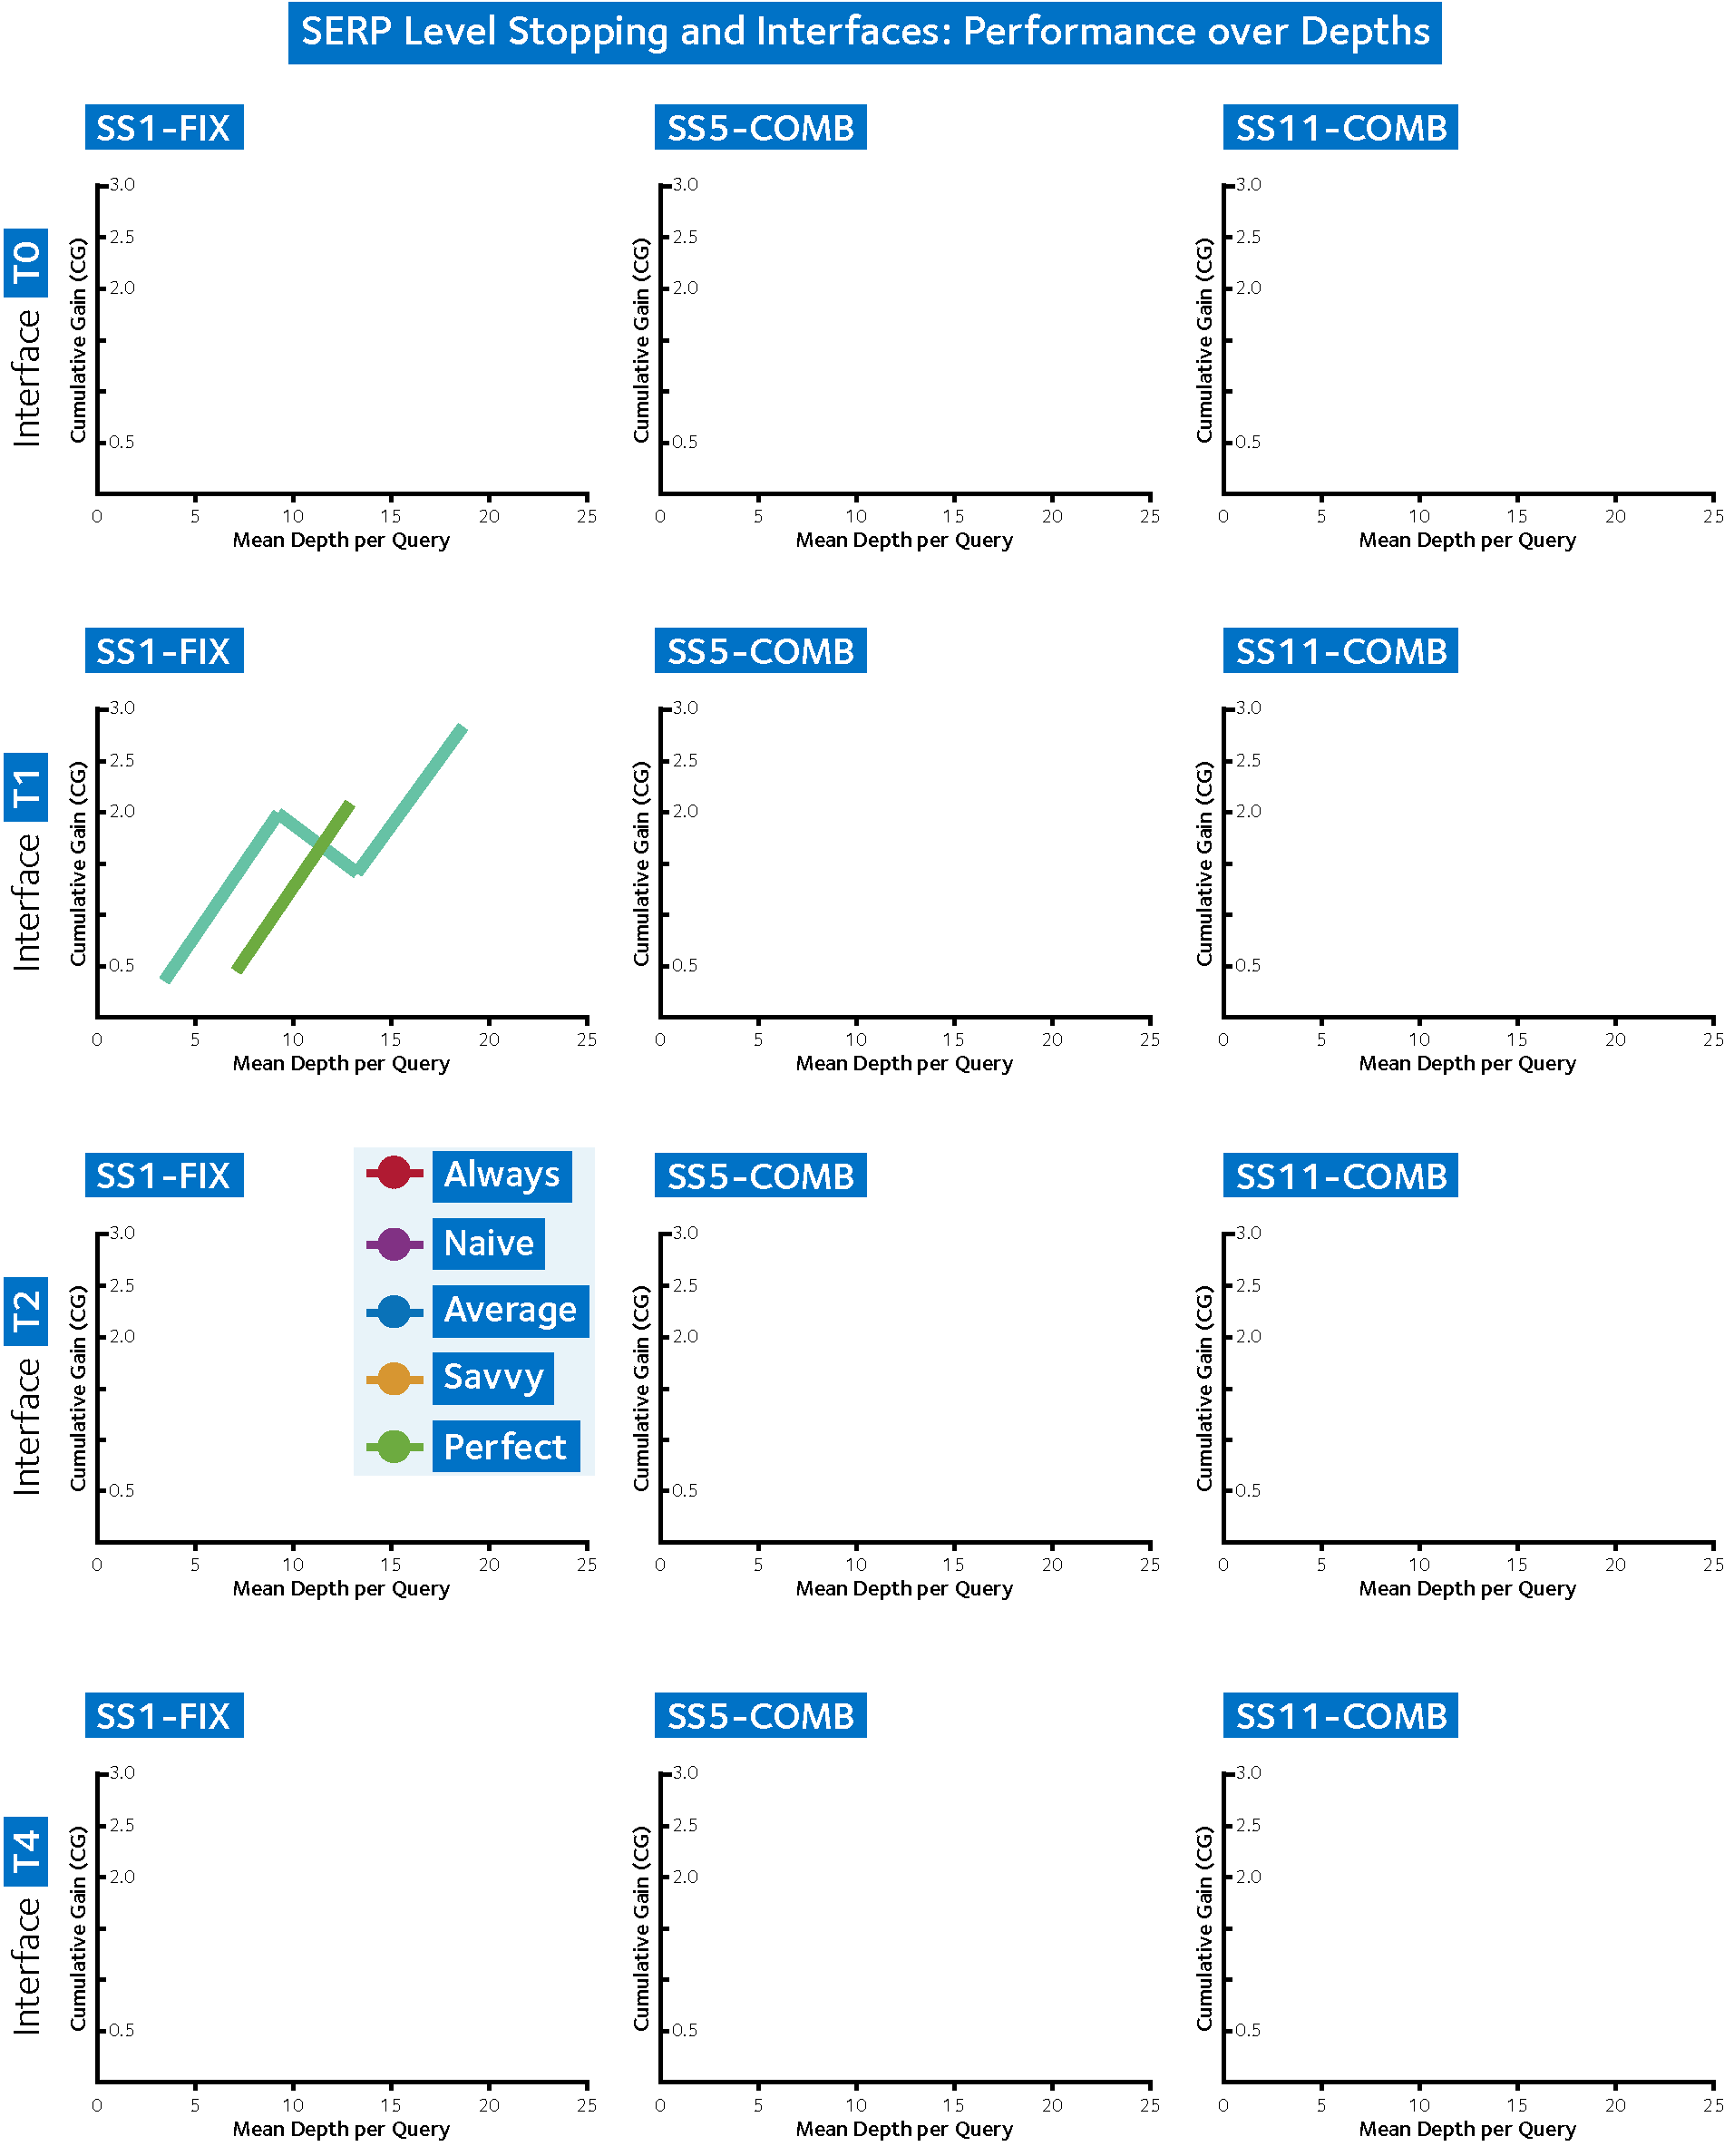
\includegraphics{figures/ch9-ch7_perf_plots.pdf}}
    \caption[Performance plots (result summaries)]{Performance plots}
    \label{fig:ch9_perf_ch7_plots}
\end{figure}

\begin{figure}[p!]
    \centering
    \resizebox{1\hsize}{!}{
    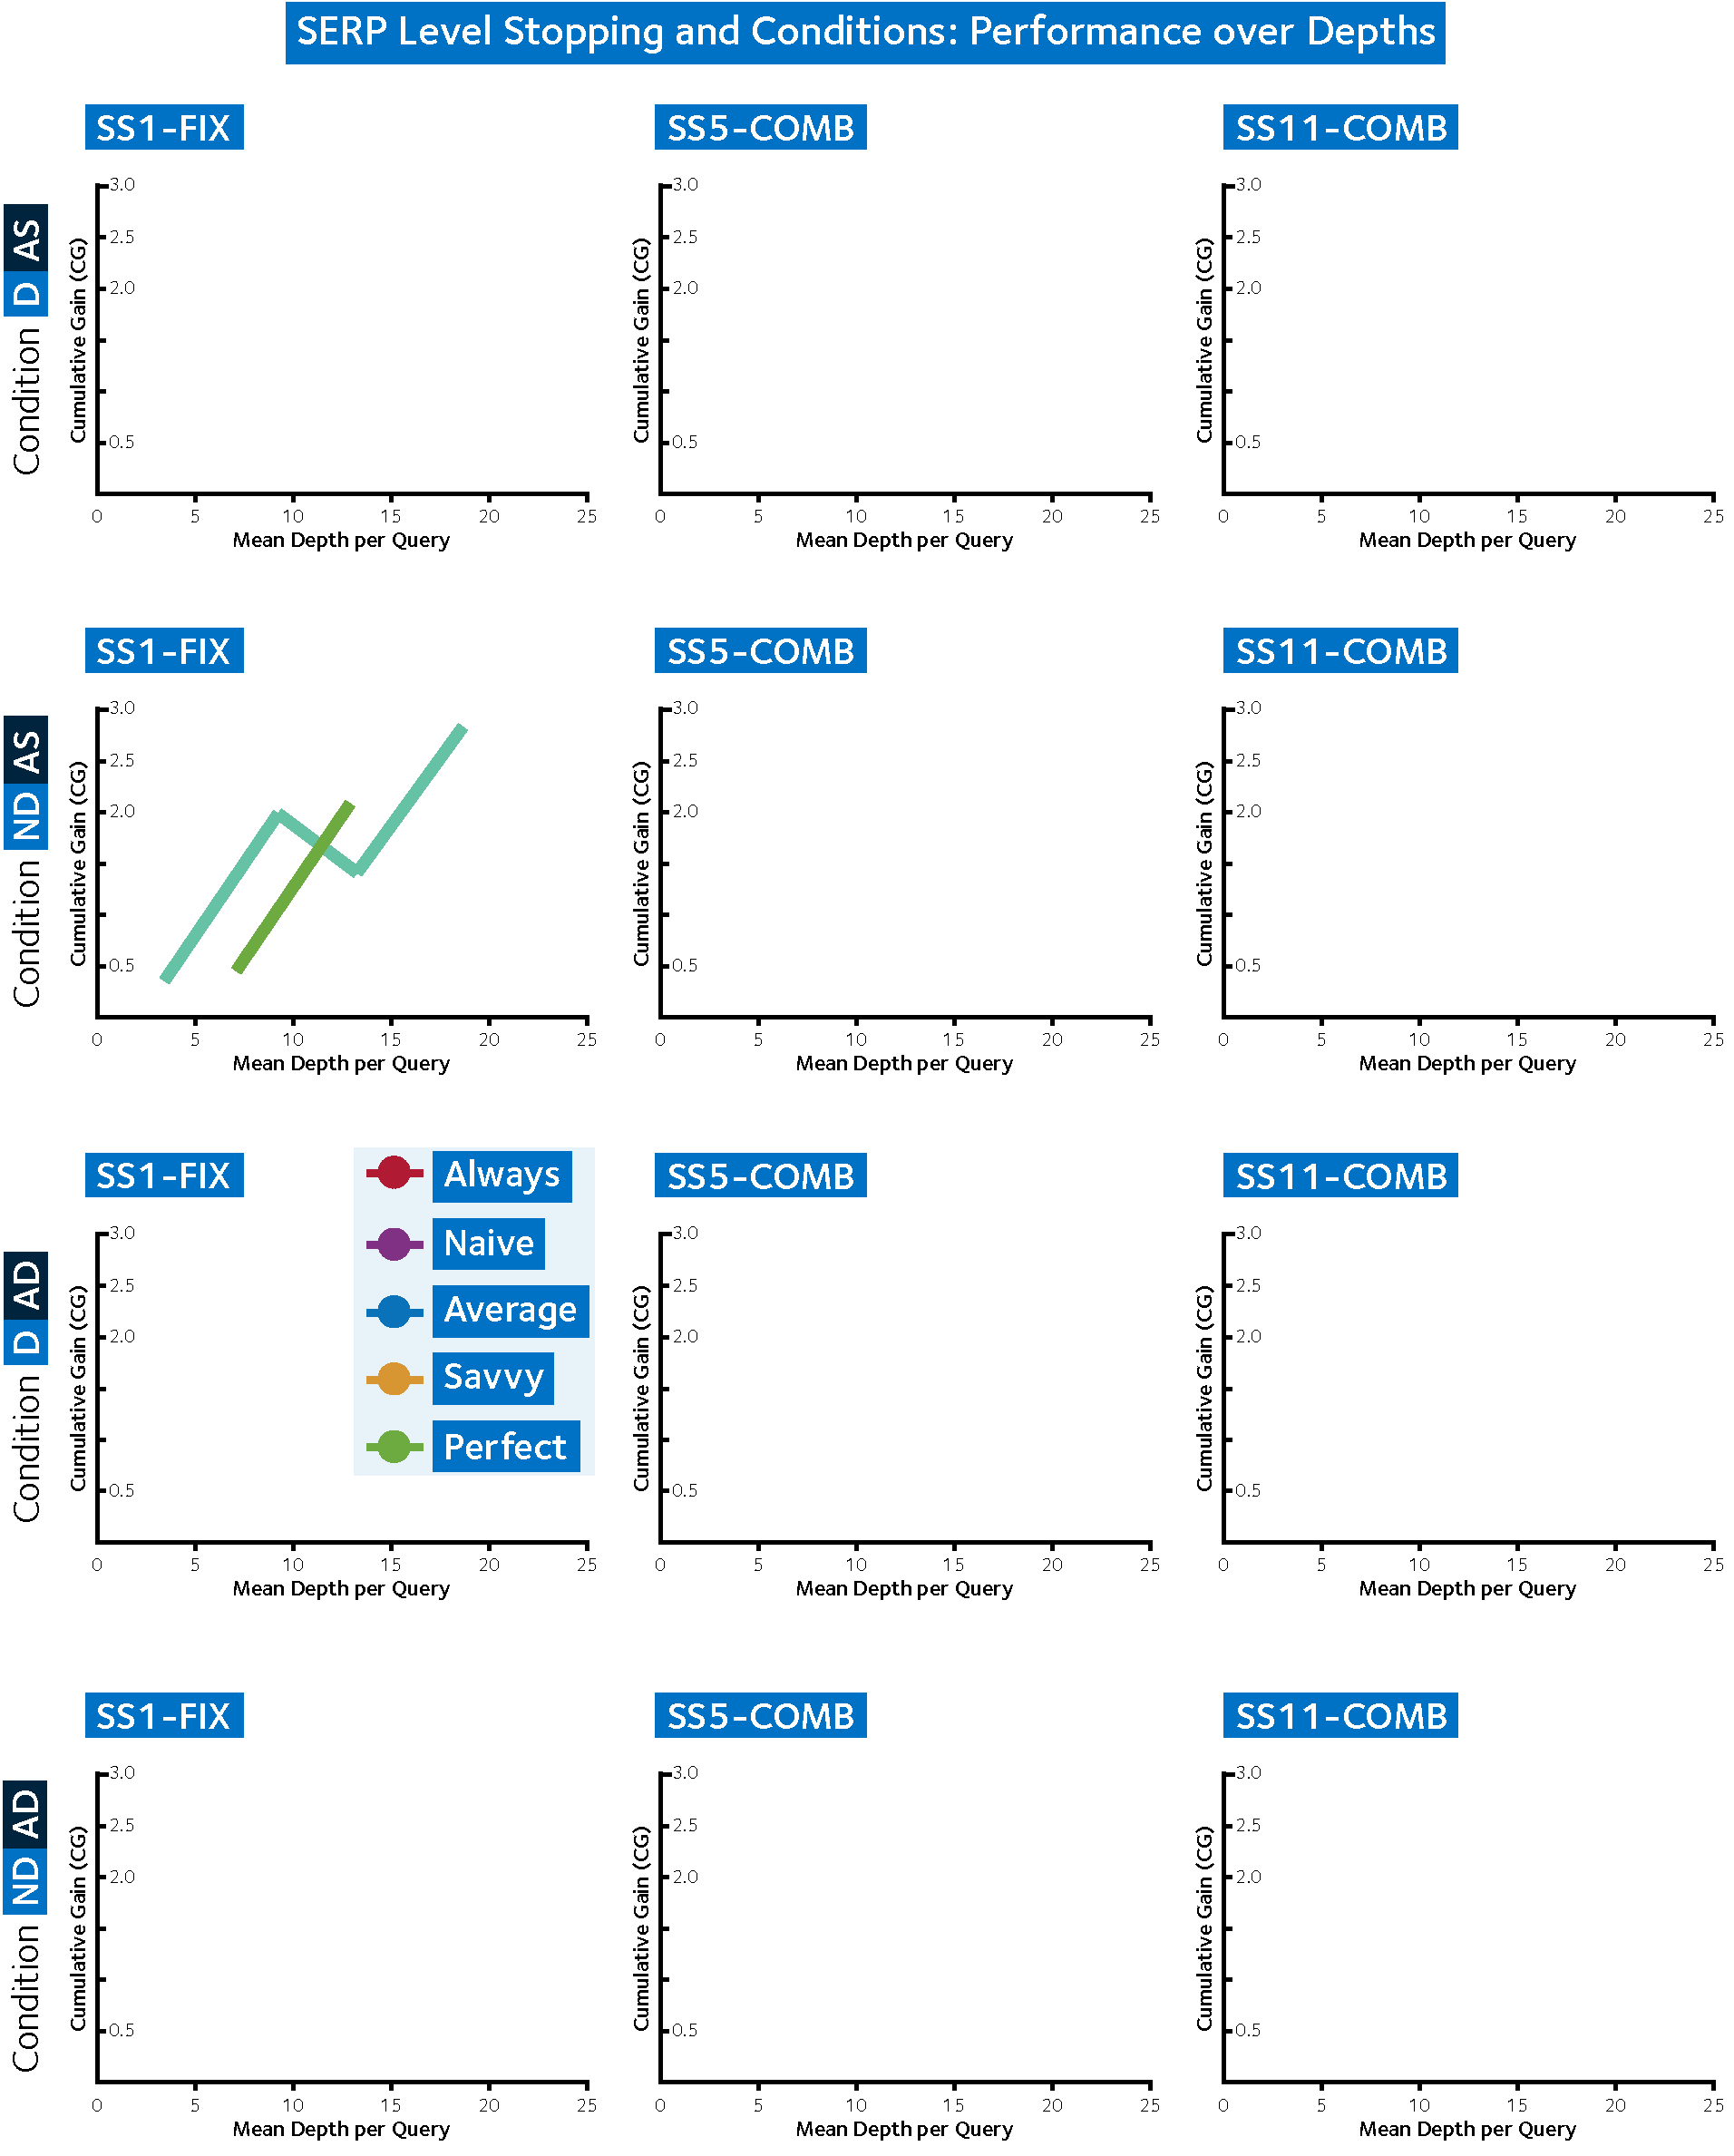
\includegraphics{figures/ch9-ch8_perf_plots.pdf}}
    \caption[Performance plots (diversification)]{Performance plots}
    \label{fig:ch9_perf_ch8_plots}
\end{figure}

\begin{table}[p!]
    \caption[Snippets Performance]{Results from the simulated what-if simulated performance runs (Chapter~\ref{chap:snippets}), showing the highest levels of~\gls{acr:cg} attained for each~\gls{acr:serp} level stopping component.}\vspace*{-2mm}
    \label{tbl:ch9_perf_ch7_table}
    \renewcommand{\arraystretch}{1.70}
    \begin{center}
        \begin{tabulary}{\textwidth}{L{0.25cm}@{\CS}L{2.15cm}@{\CS}D{0.9cm}@{\CS}D{0.9cm}@{\CS}D{0.9cm}@{\CSONEHALF}D{0.9cm}@{\CS}D{0.9cm}@{\CS}D{0.9cm}@{\CSONEHALF}D{0.9cm}@{\CS}D{0.9cm}@{\CS}D{0.9cm}@{\CSONEHALF}}
            
            & & \multicolumn{3}{@{\hskip 0pt}c@{\CSONEHALF}}{\dbluecell\small\textbf{SS1-FIX}} & \multicolumn{3}{@{\hskip 0pt}c@{\CSONEHALF}}{\dbluecell\small\textbf{SS5-COMB}} & \multicolumn{3}{@{\hskip 0pt}c@{\CSONEHALF}}{\dbluecell\small\textbf{SS11-COMB}}\\
            
            \RS & & \lbluecell\small\textbf{x\textsubscript{n}} & \lbluecell\small\textbf{DQ} & \lbluecell\small\textbf{CG} & \lbluecell\small\textbf{x\textsubscript{n}} & \lbluecell\small\textbf{DQ} & \lbluecell\small\textbf{CG} & \lbluecell\small\textbf{x\textsubscript{n}} & \lbluecell\small\textbf{DQ} & \lbluecell\small\textbf{CG} \\
            
            \RS \multirow{5}{*}{\hspace*{-2mm}\rotatebox{90}{\hspace*{-7mm}\small Interface \blueboxbold{\textbf{T0}}}} & \lbluecell\small\textbf{Always} & \cell \small \hspace*{-1mm} xx & \cell \small \hspace*{-1mm} xx & \cell \hspace*{-1mm} \small xx & \cell \small \hspace*{-1mm} xx & \cell \small \hspace*{-1mm} xx & \cell \hspace*{-1mm} \small xx & \cell \small \hspace*{-1mm} xx & \cell \small \hspace*{-1mm} xx & \cell \hspace*{-1mm} \small xx \\
            \RS  & \lbluecell\small\textbf{Perfect} & \cell \small \hspace*{-1mm} xx & \cell \small \hspace*{-1mm} xx & \cell \hspace*{-1mm} \small xx & \cell \small \hspace*{-1mm} xx & \cell \small \hspace*{-1mm} xx & \cell \hspace*{-1mm} \small xx & \cell \small \hspace*{-1mm} xx & \cell \small \hspace*{-1mm} xx & \cell \hspace*{-1mm} \small xx \\
            \RS  & \lbluecell\small\textbf{Average} & \cell \small \hspace*{-1mm} xx & \cell \small \hspace*{-1mm} xx & \cell \hspace*{-1mm} \small xx & \cell \small \hspace*{-1mm} xx & \cell \small \hspace*{-1mm} xx & \cell \hspace*{-1mm} \small xx & \cell \small \hspace*{-1mm} xx & \cell \small \hspace*{-1mm} xx & \cell \hspace*{-1mm} \small xx \\
            \RS  & \lbluecell\small\textbf{Savvy} & \cell \small \hspace*{-1mm} xx & \cell \small \hspace*{-1mm} xx & \cell \hspace*{-1mm} \small xx & \cell \small \hspace*{-1mm} xx & \cell \small \hspace*{-1mm} xx & \cell \hspace*{-1mm} \small xx & \cell \small \hspace*{-1mm} xx & \cell \small \hspace*{-1mm} xx & \cell \hspace*{-1mm} \small xx \\
            \RS  & \lbluecell\small\textbf{Na\"{i}ve} & \cell \small \hspace*{-1mm} xx & \cell \small \hspace*{-1mm} xx & \cell \hspace*{-1mm} \small xx & \cell \small \hspace*{-1mm} xx & \cell \small \hspace*{-1mm} xx & \cell \hspace*{-1mm} \small xx & \cell \small \hspace*{-1mm} xx & \cell \small \hspace*{-1mm} xx & \cell \hspace*{-1mm} \small xx \\
            
            \RS\RS\RS \multirow{5}{*}{\hspace*{-2mm}\rotatebox{90}{\hspace*{-7mm}\small Interface \blueboxbold{\textbf{T1}}}} & \lbluecell\small\textbf{Always} & \cell \small \hspace*{-1mm} xx & \cell \small \hspace*{-1mm} xx & \cell \hspace*{-1mm} \small xx & \cell \small \hspace*{-1mm} xx & \cell \small \hspace*{-1mm} xx & \cell \hspace*{-1mm} \small xx & \cell \small \hspace*{-1mm} xx & \cell \small \hspace*{-1mm} xx & \cell \hspace*{-1mm} \small xx \\
            \RS  & \lbluecell\small\textbf{Perfect} & \cell \small \hspace*{-1mm} xx & \cell \small \hspace*{-1mm} xx & \cell \hspace*{-1mm} \small xx & \cell \small \hspace*{-1mm} xx & \cell \small \hspace*{-1mm} xx & \cell \hspace*{-1mm} \small xx & \cell \small \hspace*{-1mm} xx & \cell \small \hspace*{-1mm} xx & \cell \hspace*{-1mm} \small xx \\
            \RS  & \lbluecell\small\textbf{Average} & \cell \small \hspace*{-1mm} xx & \cell \small \hspace*{-1mm} xx & \cell \hspace*{-1mm} \small xx & \cell \small \hspace*{-1mm} xx & \cell \small \hspace*{-1mm} xx & \cell \hspace*{-1mm} \small xx & \cell \small \hspace*{-1mm} xx & \cell \small \hspace*{-1mm} xx & \cell \hspace*{-1mm} \small xx \\
            \RS  & \lbluecell\small\textbf{Savvy} & \cell \small \hspace*{-1mm} xx & \cell \small \hspace*{-1mm} xx & \cell \hspace*{-1mm} \small xx & \cell \small \hspace*{-1mm} xx & \cell \small \hspace*{-1mm} xx & \cell \hspace*{-1mm} \small xx & \cell \small \hspace*{-1mm} xx & \cell \small \hspace*{-1mm} xx & \cell \hspace*{-1mm} \small xx \\
            \RS  & \lbluecell\small\textbf{Na\"{i}ve} & \cell \small \hspace*{-1mm} xx & \cell \small \hspace*{-1mm} xx & \cell \hspace*{-1mm} \small xx & \cell \small \hspace*{-1mm} xx & \cell \small \hspace*{-1mm} xx & \cell \hspace*{-1mm} \small xx & \cell \small \hspace*{-1mm} xx & \cell \small \hspace*{-1mm} xx & \cell \hspace*{-1mm} \small xx \\
            
            \RS\RS\RS \multirow{5}{*}{\hspace*{-2mm}\rotatebox{90}{\hspace*{-7mm}\small Interface \blueboxbold{\textbf{T2}}}} & \lbluecell\small\textbf{Always} & \cell \small \hspace*{-1mm} xx & \cell \small \hspace*{-1mm} xx & \cell \hspace*{-1mm} \small xx & \cell \small \hspace*{-1mm} xx & \cell \small \hspace*{-1mm} xx & \cell \hspace*{-1mm} \small xx & \cell \small \hspace*{-1mm} xx & \cell \small \hspace*{-1mm} xx & \cell \hspace*{-1mm} \small xx \\
            \RS  & \lbluecell\small\textbf{Perfect} & \cell \small \hspace*{-1mm} xx & \cell \small \hspace*{-1mm} xx & \cell \hspace*{-1mm} \small xx & \cell \small \hspace*{-1mm} xx & \cell \small \hspace*{-1mm} xx & \cell \hspace*{-1mm} \small xx & \cell \small \hspace*{-1mm} xx & \cell \small \hspace*{-1mm} xx & \cell \hspace*{-1mm} \small xx \\
            \RS  & \lbluecell\small\textbf{Average} & \cell \small \hspace*{-1mm} xx & \cell \small \hspace*{-1mm} xx & \cell \hspace*{-1mm} \small xx & \cell \small \hspace*{-1mm} xx & \cell \small \hspace*{-1mm} xx & \cell \hspace*{-1mm} \small xx & \cell \small \hspace*{-1mm} xx & \cell \small \hspace*{-1mm} xx & \cell \hspace*{-1mm} \small xx \\
            \RS  & \lbluecell\small\textbf{Savvy} & \cell \small \hspace*{-1mm} xx & \cell \small \hspace*{-1mm} xx & \cell \hspace*{-1mm} \small xx & \cell \small \hspace*{-1mm} xx & \cell \small \hspace*{-1mm} xx & \cell \hspace*{-1mm} \small xx & \cell \small \hspace*{-1mm} xx & \cell \small \hspace*{-1mm} xx & \cell \hspace*{-1mm} \small xx \\
            \RS  & \lbluecell\small\textbf{Na\"{i}ve} & \cell \small \hspace*{-1mm} xx & \cell \small \hspace*{-1mm} xx & \cell \hspace*{-1mm} \small xx & \cell \small \hspace*{-1mm} xx & \cell \small \hspace*{-1mm} xx & \cell \hspace*{-1mm} \small xx & \cell \small \hspace*{-1mm} xx & \cell \small \hspace*{-1mm} xx & \cell \hspace*{-1mm} \small xx \\
            
            \RS\RS\RS \multirow{5}{*}{\hspace*{-2mm}\rotatebox{90}{\hspace*{-7mm}\small Interface \blueboxbold{\textbf{T4}}}} & \lbluecell\small\textbf{Always} & \cell \small \hspace*{-1mm} xx & \cell \small \hspace*{-1mm} xx & \cell \hspace*{-1mm} \small xx & \cell \small \hspace*{-1mm} xx & \cell \small \hspace*{-1mm} xx & \cell \hspace*{-1mm} \small xx & \cell \small \hspace*{-1mm} xx & \cell \small \hspace*{-1mm} xx & \cell \hspace*{-1mm} \small xx \\
            \RS  & \lbluecell\small\textbf{Perfect} & \cell \small \hspace*{-1mm} xx & \cell \small \hspace*{-1mm} xx & \cell \hspace*{-1mm} \small xx & \cell \small \hspace*{-1mm} xx & \cell \small \hspace*{-1mm} xx & \cell \hspace*{-1mm} \small xx & \cell \small \hspace*{-1mm} xx & \cell \small \hspace*{-1mm} xx & \cell \hspace*{-1mm} \small xx \\
            \RS  & \lbluecell\small\textbf{Average} & \cell \small \hspace*{-1mm} xx & \cell \small \hspace*{-1mm} xx & \cell \hspace*{-1mm} \small xx & \cell \small \hspace*{-1mm} xx & \cell \small \hspace*{-1mm} xx & \cell \hspace*{-1mm} \small xx & \cell \small \hspace*{-1mm} xx & \cell \small \hspace*{-1mm} xx & \cell \hspace*{-1mm} \small xx \\
            \RS  & \lbluecell\small\textbf{Savvy} & \cell \small \hspace*{-1mm} xx & \cell \small \hspace*{-1mm} xx & \cell \hspace*{-1mm} \small xx & \cell \small \hspace*{-1mm} xx & \cell \small \hspace*{-1mm} xx & \cell \hspace*{-1mm} \small xx & \cell \small \hspace*{-1mm} xx & \cell \small \hspace*{-1mm} xx & \cell \hspace*{-1mm} \small xx \\
            \RS  & \lbluecell\small\textbf{Na\"{i}ve} & \cell \small \hspace*{-1mm} xx & \cell \small \hspace*{-1mm} xx & \cell \hspace*{-1mm} \small xx & \cell \small \hspace*{-1mm} xx & \cell \small \hspace*{-1mm} xx & \cell \hspace*{-1mm} \small xx & \cell \small \hspace*{-1mm} xx & \cell \small \hspace*{-1mm} xx & \cell \hspace*{-1mm} \small xx \\

        \end{tabulary}
        \end{center}
    \end{table}



\begin{table}[p!]
    \caption[Diversification Performance]{Results from the simulated what-if simulated performance runs (Chapter~\ref{chap:diversity}), showing the highest levels of~\gls{acr:cg} attained for each~\gls{acr:serp} level stopping component.}\vspace*{-2mm}
    \label{tbl:ch9_perf_ch8_table}
    \renewcommand{\arraystretch}{1.70}
    \begin{center}
        \begin{tabulary}{\textwidth}{L{0.25cm}@{\CS}L{2.15cm}@{\CS}D{0.9cm}@{\CS}D{0.9cm}@{\CS}D{0.9cm}@{\CSONEHALF}D{0.9cm}@{\CS}D{0.9cm}@{\CS}D{0.9cm}@{\CSONEHALF}D{0.9cm}@{\CS}D{0.9cm}@{\CS}D{0.9cm}@{\CSONEHALF}}
            
            & & \multicolumn{3}{@{\hskip 0pt}c@{\CSONEHALF}}{\dbluecell\small\textbf{SS1-FIX}} & \multicolumn{3}{@{\hskip 0pt}c@{\CSONEHALF}}{\dbluecell\small\textbf{SS5-COMB}} & \multicolumn{3}{@{\hskip 0pt}c@{\CSONEHALF}}{\dbluecell\small\textbf{SS11-COMB}}\\
            
            \RS & & \lbluecell\small\textbf{x\textsubscript{n}} & \lbluecell\small\textbf{DQ} & \lbluecell\small\textbf{CG} & \lbluecell\small\textbf{x\textsubscript{n}} & \lbluecell\small\textbf{DQ} & \lbluecell\small\textbf{CG} & \lbluecell\small\textbf{x\textsubscript{n}} & \lbluecell\small\textbf{DQ} & \lbluecell\small\textbf{CG} \\
            
            \RS \multirow{5}{*}{\hspace*{-2mm}\rotatebox{90}{\hspace*{-7mm}\small Condition \textbf{\dualbluebox{D}{AS}}}} & \lbluecell\small\textbf{Always} & \cell \small \hspace*{-1mm} xx & \cell \small \hspace*{-1mm} xx & \cell \hspace*{-1mm} \small xx & \cell \small \hspace*{-1mm} xx & \cell \small \hspace*{-1mm} xx & \cell \hspace*{-1mm} \small xx & \cell \small \hspace*{-1mm} xx & \cell \small \hspace*{-1mm} xx & \cell \hspace*{-1mm} \small xx \\
            \RS  & \lbluecell\small\textbf{Perfect} & \cell \small \hspace*{-1mm} xx & \cell \small \hspace*{-1mm} xx & \cell \hspace*{-1mm} \small xx & \cell \small \hspace*{-1mm} xx & \cell \small \hspace*{-1mm} xx & \cell \hspace*{-1mm} \small xx & \cell \small \hspace*{-1mm} xx & \cell \small \hspace*{-1mm} xx & \cell \hspace*{-1mm} \small xx \\
            \RS  & \lbluecell\small\textbf{Average} & \cell \small \hspace*{-1mm} xx & \cell \small \hspace*{-1mm} xx & \cell \hspace*{-1mm} \small xx & \cell \small \hspace*{-1mm} xx & \cell \small \hspace*{-1mm} xx & \cell \hspace*{-1mm} \small xx & \cell \small \hspace*{-1mm} xx & \cell \small \hspace*{-1mm} xx & \cell \hspace*{-1mm} \small xx \\
            \RS  & \lbluecell\small\textbf{Savvy} & \cell \small \hspace*{-1mm} xx & \cell \small \hspace*{-1mm} xx & \cell \hspace*{-1mm} \small xx & \cell \small \hspace*{-1mm} xx & \cell \small \hspace*{-1mm} xx & \cell \hspace*{-1mm} \small xx & \cell \small \hspace*{-1mm} xx & \cell \small \hspace*{-1mm} xx & \cell \hspace*{-1mm} \small xx \\
            \RS  & \lbluecell\small\textbf{Na\"{i}ve} & \cell \small \hspace*{-1mm} xx & \cell \small \hspace*{-1mm} xx & \cell \hspace*{-1mm} \small xx & \cell \small \hspace*{-1mm} xx & \cell \small \hspace*{-1mm} xx & \cell \hspace*{-1mm} \small xx & \cell \small \hspace*{-1mm} xx & \cell \small \hspace*{-1mm} xx & \cell \hspace*{-1mm} \small xx \\
            
            \RS\RS\RS \multirow{5}{*}{\hspace*{-2mm}\rotatebox{90}{\hspace*{-7mm}\small Condition \textbf{\dualbluebox{ND}{AS}}}} & \lbluecell\small\textbf{Always} & \cell \small \hspace*{-1mm} xx & \cell \small \hspace*{-1mm} xx & \cell \hspace*{-1mm} \small xx & \cell \small \hspace*{-1mm} xx & \cell \small \hspace*{-1mm} xx & \cell \hspace*{-1mm} \small xx & \cell \small \hspace*{-1mm} xx & \cell \small \hspace*{-1mm} xx & \cell \hspace*{-1mm} \small xx \\
            \RS  & \lbluecell\small\textbf{Perfect} & \cell \small \hspace*{-1mm} xx & \cell \small \hspace*{-1mm} xx & \cell \hspace*{-1mm} \small xx & \cell \small \hspace*{-1mm} xx & \cell \small \hspace*{-1mm} xx & \cell \hspace*{-1mm} \small xx & \cell \small \hspace*{-1mm} xx & \cell \small \hspace*{-1mm} xx & \cell \hspace*{-1mm} \small xx \\
            \RS  & \lbluecell\small\textbf{Average} & \cell \small \hspace*{-1mm} xx & \cell \small \hspace*{-1mm} xx & \cell \hspace*{-1mm} \small xx & \cell \small \hspace*{-1mm} xx & \cell \small \hspace*{-1mm} xx & \cell \hspace*{-1mm} \small xx & \cell \small \hspace*{-1mm} xx & \cell \small \hspace*{-1mm} xx & \cell \hspace*{-1mm} \small xx \\
            \RS  & \lbluecell\small\textbf{Savvy} & \cell \small \hspace*{-1mm} xx & \cell \small \hspace*{-1mm} xx & \cell \hspace*{-1mm} \small xx & \cell \small \hspace*{-1mm} xx & \cell \small \hspace*{-1mm} xx & \cell \hspace*{-1mm} \small xx & \cell \small \hspace*{-1mm} xx & \cell \small \hspace*{-1mm} xx & \cell \hspace*{-1mm} \small xx \\
            \RS  & \lbluecell\small\textbf{Na\"{i}ve} & \cell \small \hspace*{-1mm} xx & \cell \small \hspace*{-1mm} xx & \cell \hspace*{-1mm} \small xx & \cell \small \hspace*{-1mm} xx & \cell \small \hspace*{-1mm} xx & \cell \hspace*{-1mm} \small xx & \cell \small \hspace*{-1mm} xx & \cell \small \hspace*{-1mm} xx & \cell \hspace*{-1mm} \small xx \\
            
            \RS\RS\RS \multirow{5}{*}{\hspace*{-2mm}\rotatebox{90}{\hspace*{-7mm}\small Condition \textbf{\dualbluebox{D}{AD}}}} & \lbluecell\small\textbf{Always} & \cell \small \hspace*{-1mm} xx & \cell \small \hspace*{-1mm} xx & \cell \hspace*{-1mm} \small xx & \cell \small \hspace*{-1mm} xx & \cell \small \hspace*{-1mm} xx & \cell \hspace*{-1mm} \small xx & \cell \small \hspace*{-1mm} xx & \cell \small \hspace*{-1mm} xx & \cell \hspace*{-1mm} \small xx \\
            \RS  & \lbluecell\small\textbf{Perfect} & \cell \small \hspace*{-1mm} xx & \cell \small \hspace*{-1mm} xx & \cell \hspace*{-1mm} \small xx & \cell \small \hspace*{-1mm} xx & \cell \small \hspace*{-1mm} xx & \cell \hspace*{-1mm} \small xx & \cell \small \hspace*{-1mm} xx & \cell \small \hspace*{-1mm} xx & \cell \hspace*{-1mm} \small xx \\
            \RS  & \lbluecell\small\textbf{Average} & \cell \small \hspace*{-1mm} xx & \cell \small \hspace*{-1mm} xx & \cell \hspace*{-1mm} \small xx & \cell \small \hspace*{-1mm} xx & \cell \small \hspace*{-1mm} xx & \cell \hspace*{-1mm} \small xx & \cell \small \hspace*{-1mm} xx & \cell \small \hspace*{-1mm} xx & \cell \hspace*{-1mm} \small xx \\
            \RS  & \lbluecell\small\textbf{Savvy} & \cell \small \hspace*{-1mm} xx & \cell \small \hspace*{-1mm} xx & \cell \hspace*{-1mm} \small xx & \cell \small \hspace*{-1mm} xx & \cell \small \hspace*{-1mm} xx & \cell \hspace*{-1mm} \small xx & \cell \small \hspace*{-1mm} xx & \cell \small \hspace*{-1mm} xx & \cell \hspace*{-1mm} \small xx \\
            \RS  & \lbluecell\small\textbf{Na\"{i}ve} & \cell \small \hspace*{-1mm} xx & \cell \small \hspace*{-1mm} xx & \cell \hspace*{-1mm} \small xx & \cell \small \hspace*{-1mm} xx & \cell \small \hspace*{-1mm} xx & \cell \hspace*{-1mm} \small xx & \cell \small \hspace*{-1mm} xx & \cell \small \hspace*{-1mm} xx & \cell \hspace*{-1mm} \small xx \\
            
            \RS\RS\RS \multirow{5}{*}{\hspace*{-2mm}\rotatebox{90}{\hspace*{-7mm}\small Condition \textbf{\dualbluebox{ND}{AD}}}} & \lbluecell\small\textbf{Always} & \cell \small \hspace*{-1mm} xx & \cell \small \hspace*{-1mm} xx & \cell \hspace*{-1mm} \small xx & \cell \small \hspace*{-1mm} xx & \cell \small \hspace*{-1mm} xx & \cell \hspace*{-1mm} \small xx & \cell \small \hspace*{-1mm} xx & \cell \small \hspace*{-1mm} xx & \cell \hspace*{-1mm} \small xx \\
            \RS  & \lbluecell\small\textbf{Perfect} & \cell \small \hspace*{-1mm} xx & \cell \small \hspace*{-1mm} xx & \cell \hspace*{-1mm} \small xx & \cell \small \hspace*{-1mm} xx & \cell \small \hspace*{-1mm} xx & \cell \hspace*{-1mm} \small xx & \cell \small \hspace*{-1mm} xx & \cell \small \hspace*{-1mm} xx & \cell \hspace*{-1mm} \small xx \\
            \RS  & \lbluecell\small\textbf{Average} & \cell \small \hspace*{-1mm} xx & \cell \small \hspace*{-1mm} xx & \cell \hspace*{-1mm} \small xx & \cell \small \hspace*{-1mm} xx & \cell \small \hspace*{-1mm} xx & \cell \hspace*{-1mm} \small xx & \cell \small \hspace*{-1mm} xx & \cell \small \hspace*{-1mm} xx & \cell \hspace*{-1mm} \small xx \\
            \RS  & \lbluecell\small\textbf{Savvy} & \cell \small \hspace*{-1mm} xx & \cell \small \hspace*{-1mm} xx & \cell \hspace*{-1mm} \small xx & \cell \small \hspace*{-1mm} xx & \cell \small \hspace*{-1mm} xx & \cell \hspace*{-1mm} \small xx & \cell \small \hspace*{-1mm} xx & \cell \small \hspace*{-1mm} xx & \cell \hspace*{-1mm} \small xx \\
            \RS  & \lbluecell\small\textbf{Na\"{i}ve} & \cell \small \hspace*{-1mm} xx & \cell \small \hspace*{-1mm} xx & \cell \hspace*{-1mm} \small xx & \cell \small \hspace*{-1mm} xx & \cell \small \hspace*{-1mm} xx & \cell \hspace*{-1mm} \small xx & \cell \small \hspace*{-1mm} xx & \cell \small \hspace*{-1mm} xx & \cell \hspace*{-1mm} \small xx \\

        \end{tabulary}
        \end{center}
    \end{table}

\subsection{Real-World Comparisons}

\begin{figure}[p!]
    \centering
    \resizebox{1\hsize}{!}{
    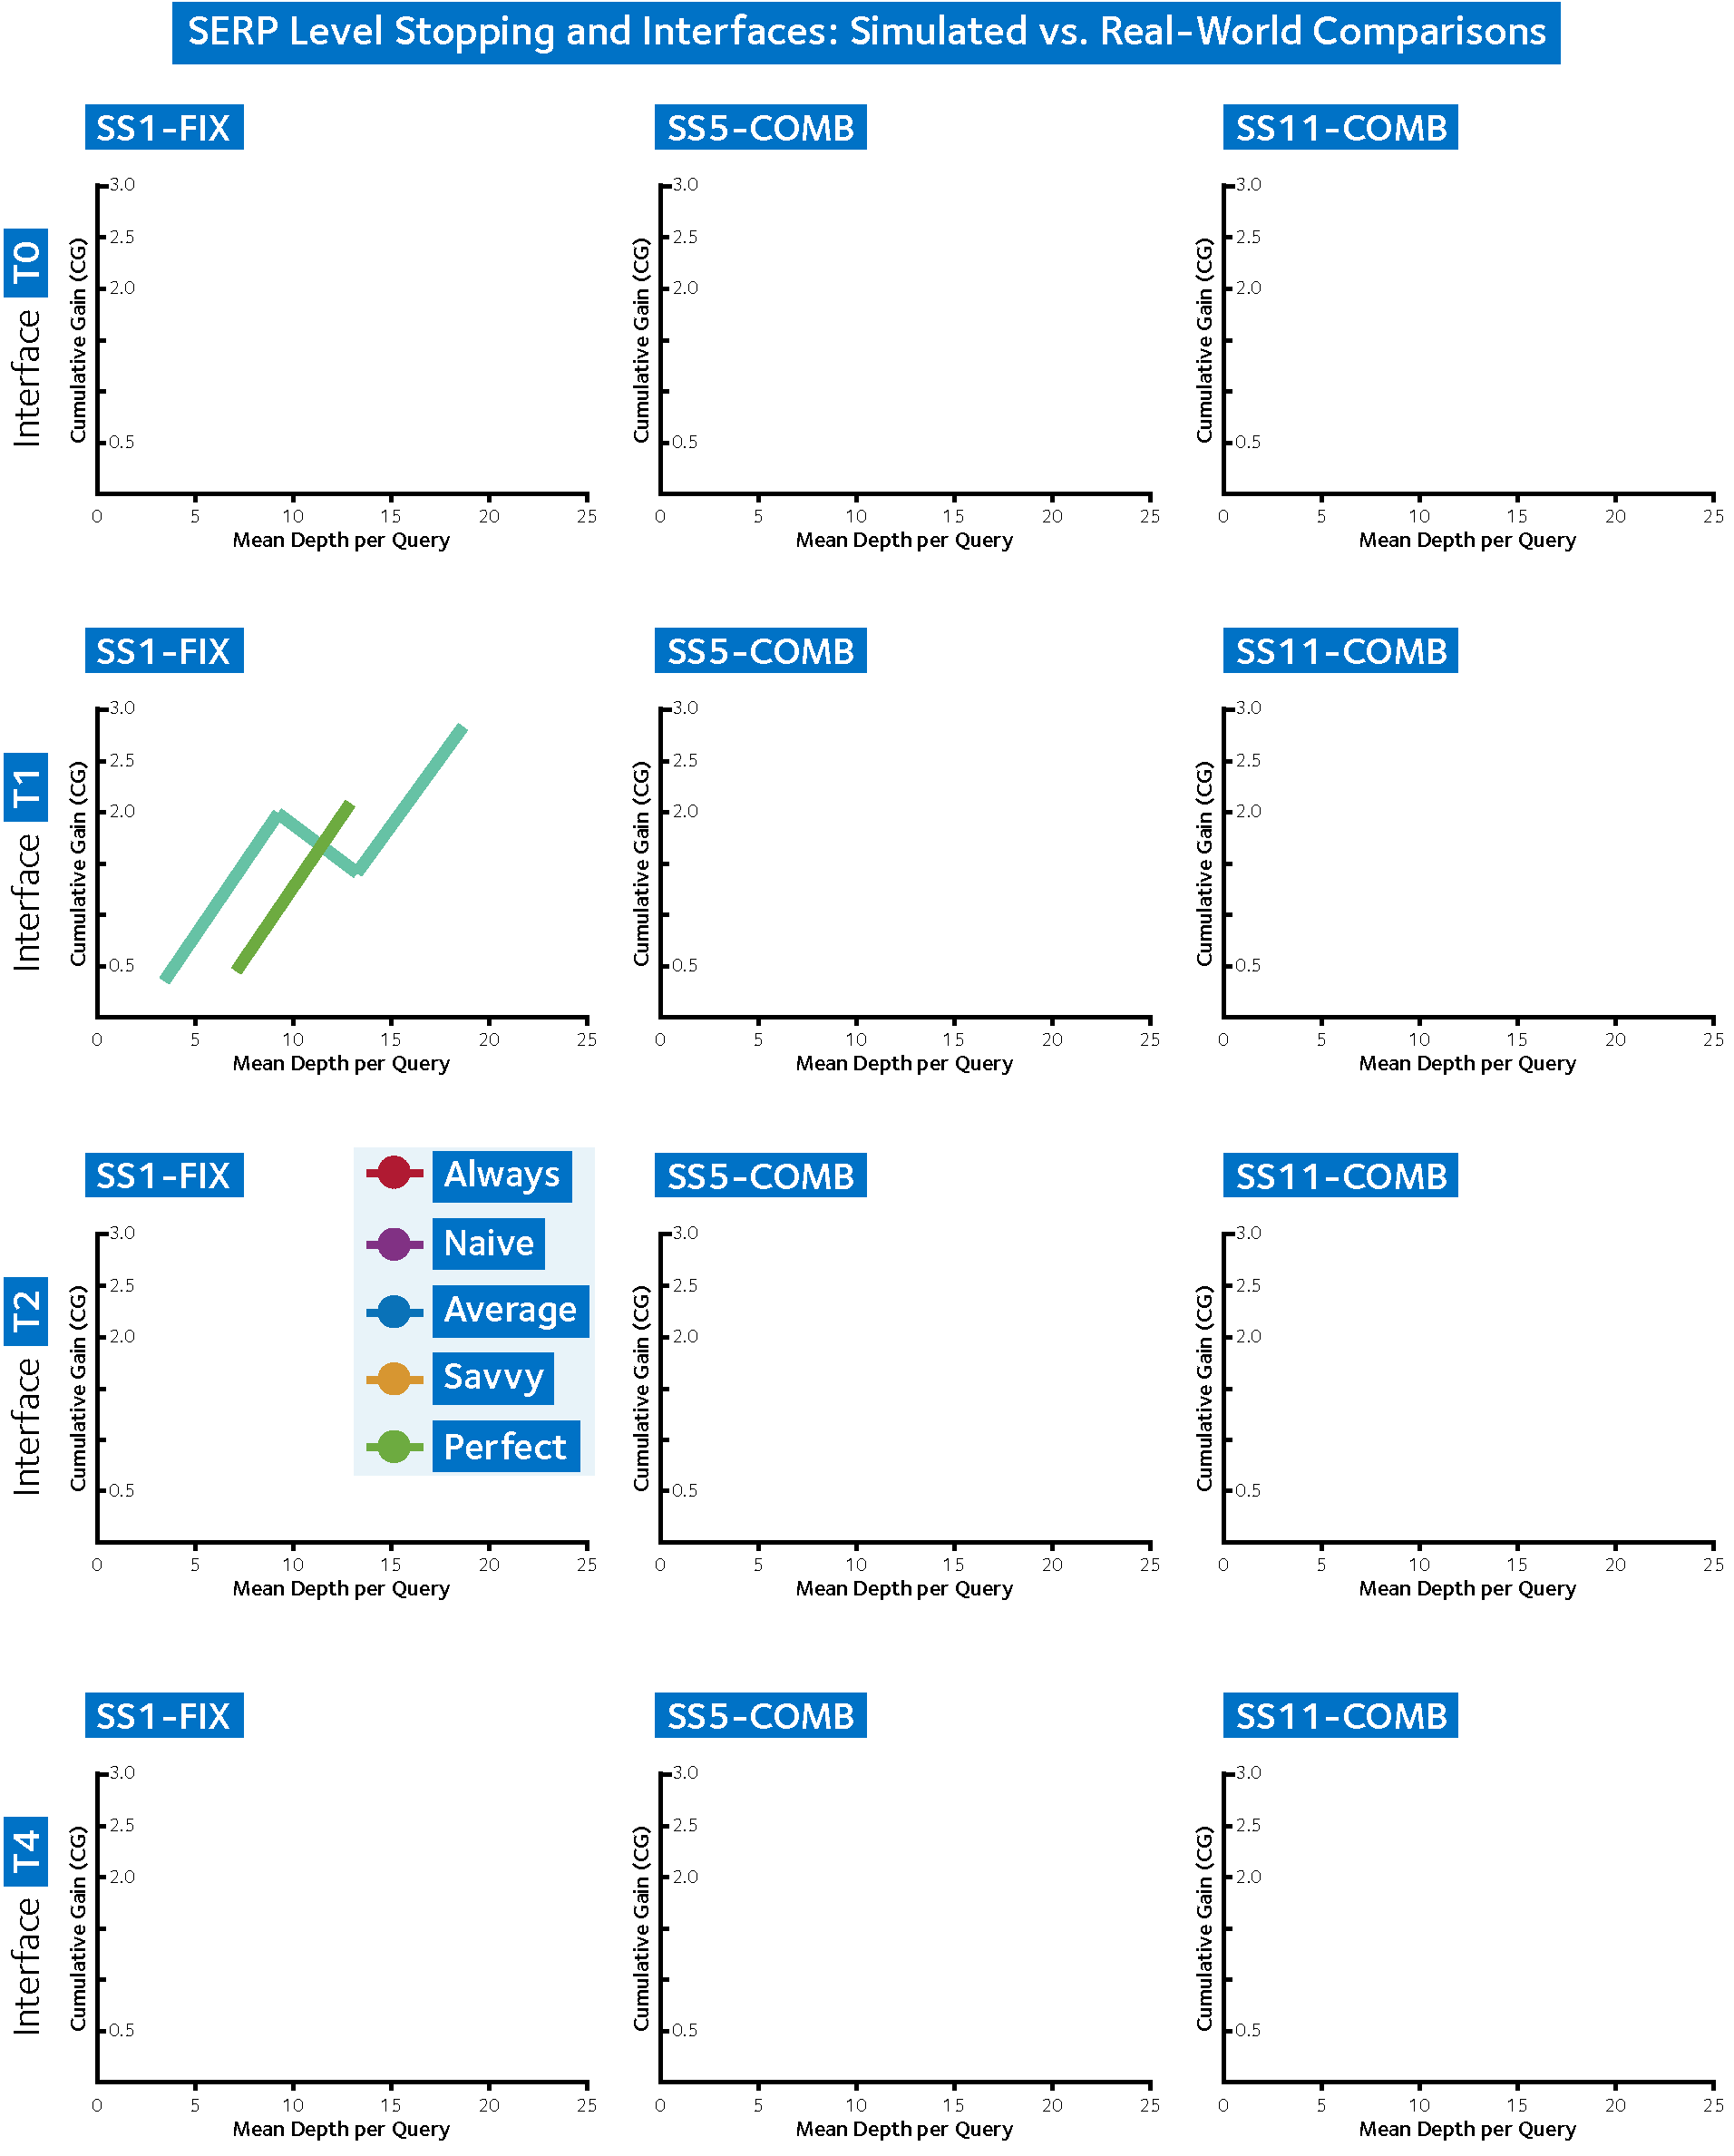
\includegraphics{figures/ch9-ch7_comparison_plots.pdf}}
    \caption[Comparison plots (result summaries)]{Comparison plots}
    \label{fig:ch9_comparison_ch7_plots}
\end{figure}

\begin{figure}[p!]
    \centering
    \resizebox{1\hsize}{!}{
    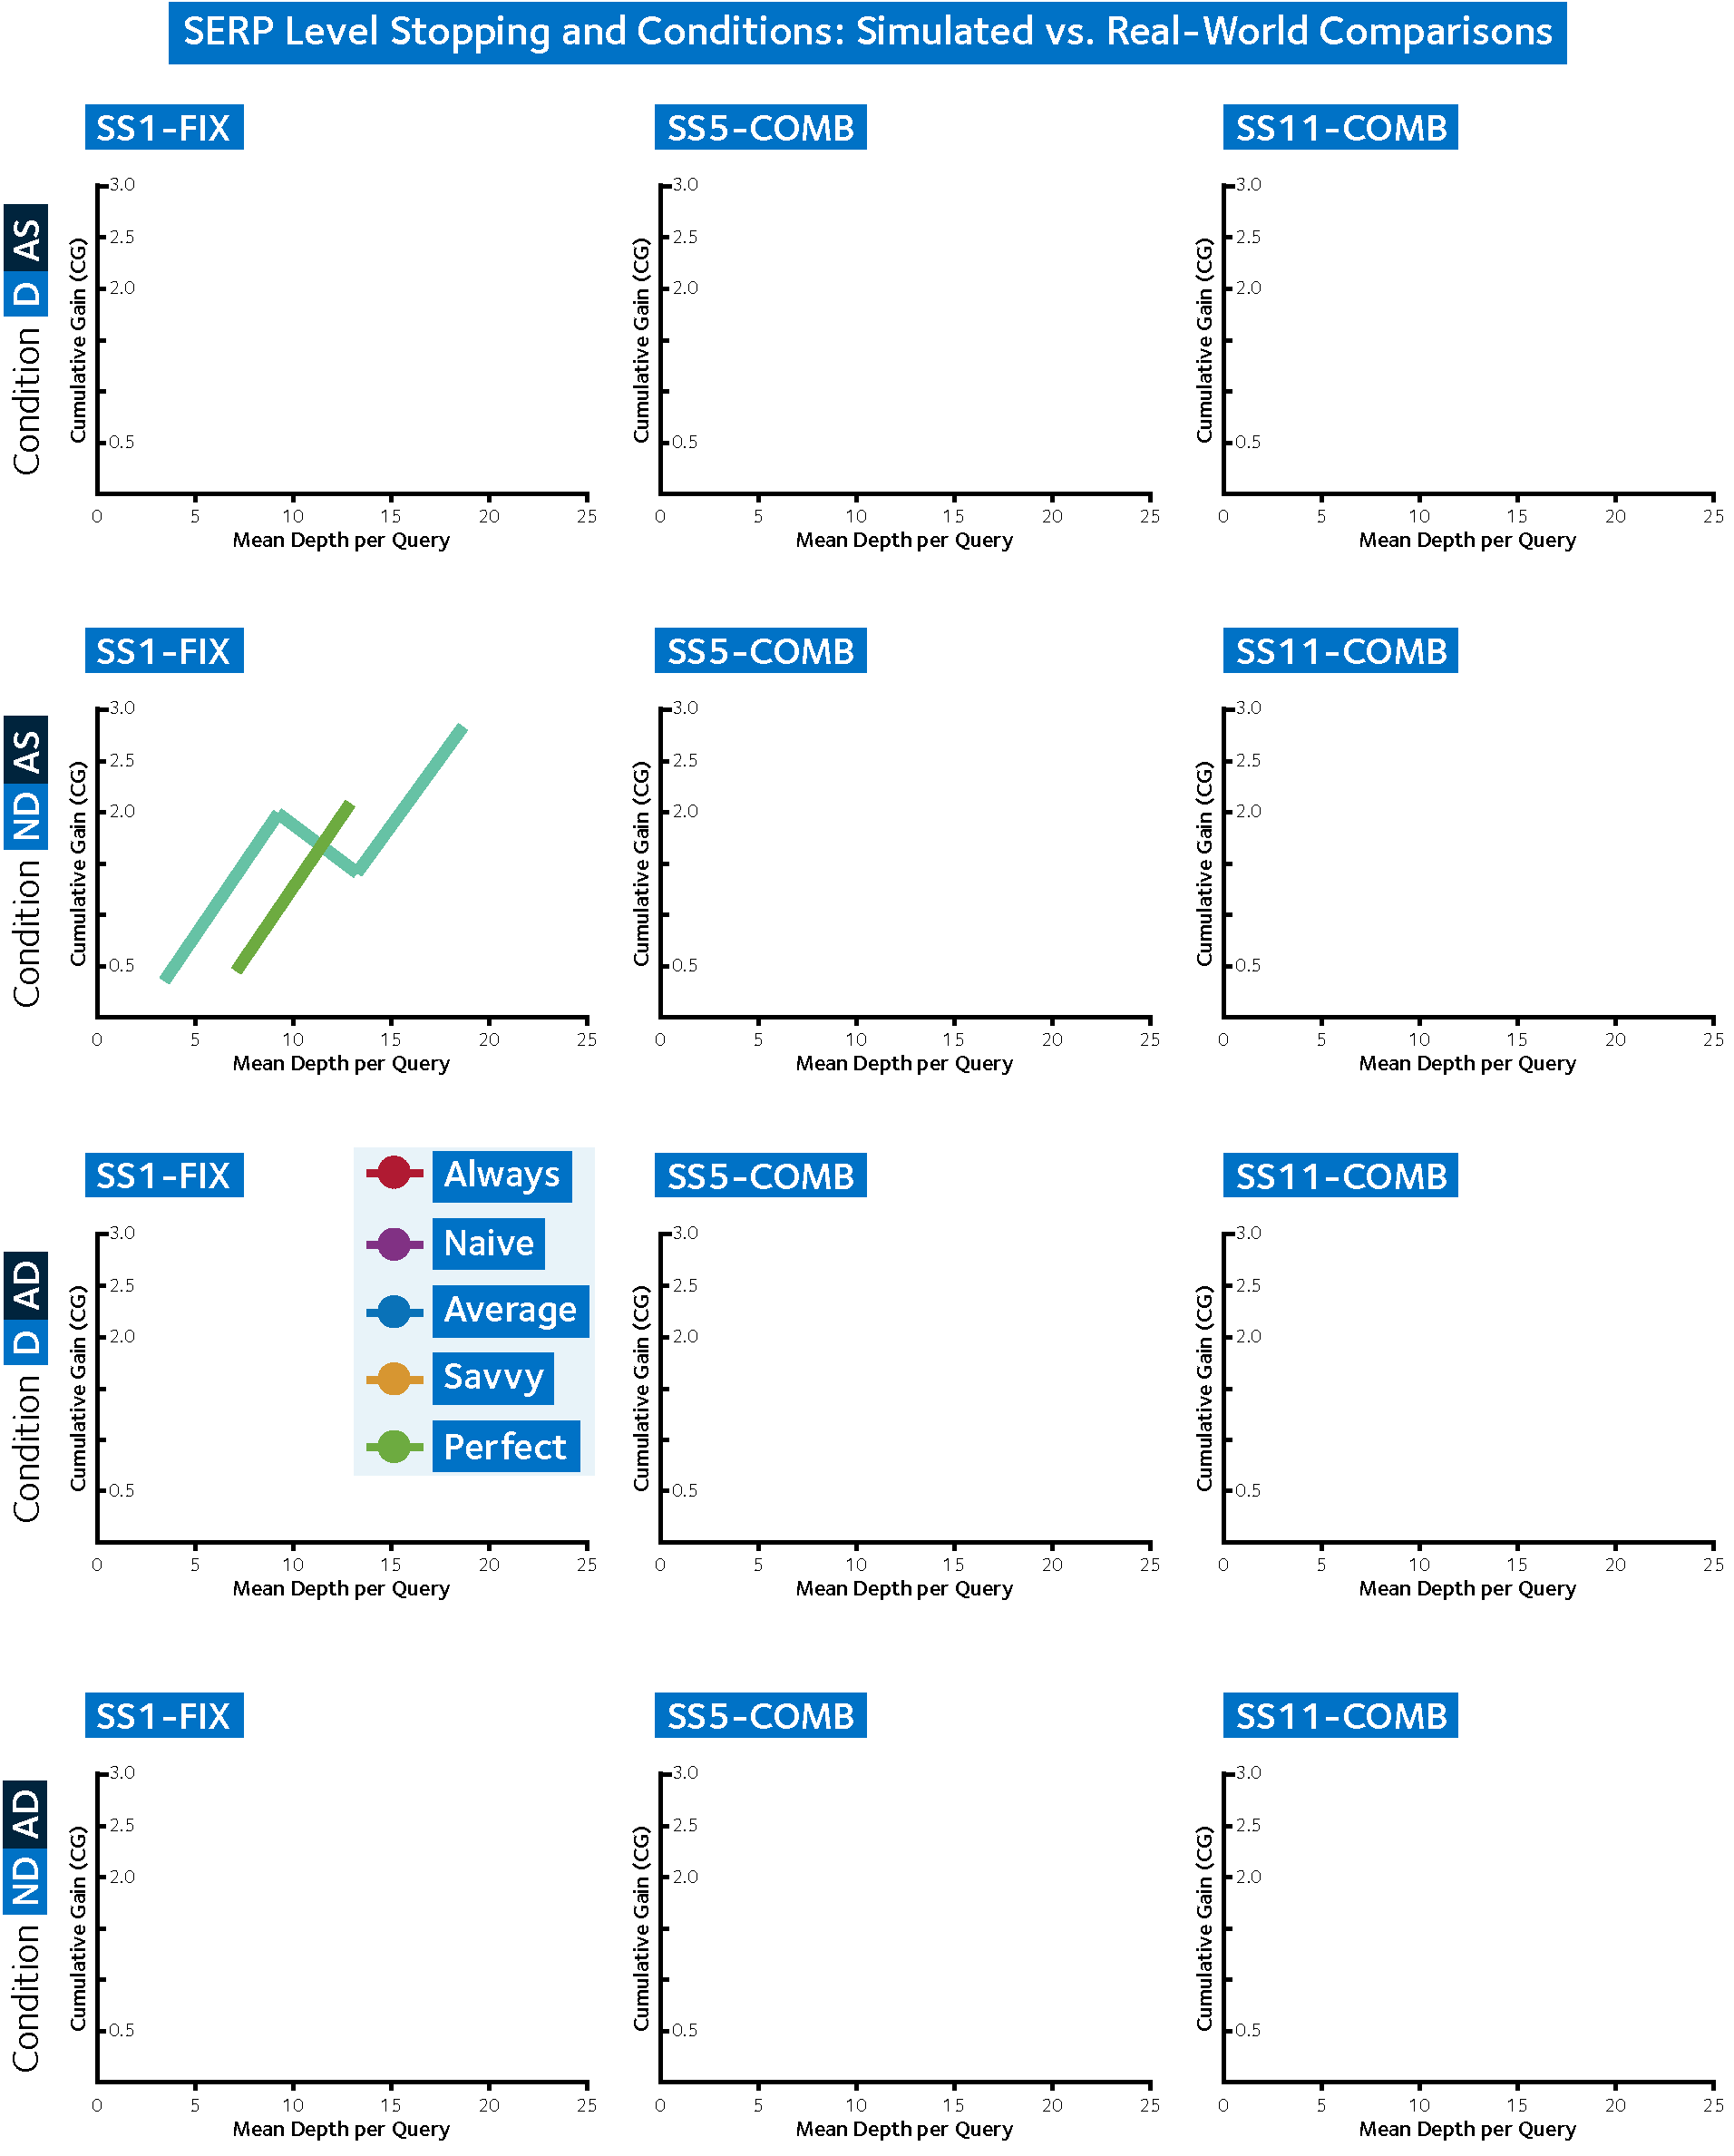
\includegraphics{figures/ch9-ch8_comparison_plots.pdf}}
    \caption[Comparison plots (diversification)]{Comparison plots}
    \label{fig:ch9_comparison_ch8_plots}
\end{figure}

\section{Chapter Summary}